% !TEX root = memoire/main.tex

\chapter{Assimilation de données pour la construction d'un jumeau numérique}~\label{sec:da}

\section{Introduction}~\label{sec:intro_da}

La construction d'un système expert ou jumeau numérique a besoin de méthode qui puissent faire le lien entre observations et l'état de notre simulation.

En effet, les solutions calculées par les modèles numériques comportent des erreurs qu'il est crucial de comprendre, de quantifier et de réduire.

Cette incertitude peut se manifester sous diverses formes, telles que l'ambiguïté des valeurs des paramètres du modèle, l'imprécision des conditions initiales, ou l'incertitude dans la définition des conditions aux limites ou des forces extérieures. De plus, bien que les modèles numériques intègrent généralement des principes physiques essentiels, ils impliquent certaines simplifications. L'erreur numérique apparaît en raison de l'algorithme et de la discrétisation. Elle s'étend également à l'incertitude associée aux futures mesures expérimentales calibrant les modèles numériques.

En revanche, les approches stochastiques vont au-delà de la simple estimation de l'état ; elles quantifient l'incertitude associée aux états estimés. Cela est crucial, en particulier dans les systèmes dynamiques et incertains, où la reconnaissance et la caractérisation de l'incertitude deviennent primordiales pour une prise de décision fiable et l'amélioration des modèles. Dans cette approche, l'estimation est mise à jour séquentiellement en fonction des observations précédentes et actuelles. Le processus d'assimilation est réalisé dans un cadre bayésien avec une étape de prévision et une étape d'analyse. Le filtre de Kalman est un exemple de formulation séquentielle qui considère un modèle linéaire et des hypothèses de distribution gaussienne. Cependant, des filtres plus avancés ont été introduits pour s'adapter aux distributions non linéaires et arbitraires. L'un des filtres bayésiens les plus populaires est sans doute l'Ensemble Kalman Filter, introduit par Evensen, principalement en raison de son adaptabilité aux problèmes de haute dimension avec tout modèle d'évolution. Il consiste à approximer la distribution de probabilité d'un état grâce à un ensemble de simulations appelées particules ou membres.

\section{Formalisme du problème d'assimilation}

Nous décrirons le problème d'assimilation sous sa forme d'inférence bayésienne. Suivant différentes hypothèses, nous montrerons qu'elle s'exprime alors sous des formes variées.

\subsection{Définition de l'état}

Nous définissons un état $\bm z_k$ comme la variable d'\textit{état} qui représente complètement la connaissance du système à l'instant $t_k \in \mathbb R^+$. La dynamique de l'état du système au cours du temps est obtenu grâce un modèle $\mathcal{M}$ qui décrit l'évolution du système.
Nous noterons $\mathcal Z_k = \{\bz_0, \dots, \bz_k\}$ la trajectoire du modèle jusqu'au pas de temps $t_k$.
Nous supposerons que le modèle admet des incertitudes. Celle-ci sont issues de

\begin{itemize}
    \item \textbf{L'erreur de discrétisation} dans l'espace et le temps. Soit $\bz^c$ l'état réel continu. Le modèle numérique ne traite que des représentations discrètes du champ physique. Ainsi, c'est non pas l'état $\bm x^c$ qui est estimé mais une projection dans l'espace de discrétisation. On estimera $\bz^t = \Pi(\bz^c)$, où $\Pi$ est un projecteur sur l'espace de discrétisation. On parle ici d'erreur de \textit{représentativité}.
    \item \textbf{L'erreur de modèle}. C'est un modèle numérique qui calcule l'évolution de l'état simulé. Tout modèle étant imparfait, toutes les physiques ne peuvent êter prises en compte. C'est une erreur qui tient compte de la mauvaise représentation de l'évolution du système mais également de sa discrétisation.
    \item \textbf{L'erreur de données} Le modèle mathématique doit être complété par des données et des paramètres spécifiant les caractéristiques physiques du système simulé parmi la classe des systèmes représentés par le modèle. Ces données peuvent concerner la géométrie du système, les conditions aux limites et initiales, ainsi que les forçages externes. Les paramètres peuvent être des constantes physiques ou des constantes du modèle prescrivant les lois constitutives du système. L'utilisation de données qui ne reflètent que partiellement la nature du système exact induit des erreurs supplémentaires, appelées erreurs de données, sur la prédiction.
\end{itemize}

Ainsi, nous traiterons l'état comme une variable aléatoire tel que à laquelle nous lui associerons une incertitude à la prédiction $\bm \eta_k$

\begin{equation*}
    \bm z_k \mathcal{M}(\bz_0, t_k ; \bm \theta) + \eta_k.
\end{equation*}
où $\bm \theta$ sont l'ensemble des paramètres du modèle et $\bm z_0$ l'état initial.

\subsection{Définition des obervations}
A l'équation d'évolution, nous supposons également connue une équation d'émission ou équation d'observation. Celle-ci relie l'état à l'espace de mesures. On définie $\mathcal{D}_k$ les mesures prédites par la fenêtre d'état $\mathcal{Z}_k$. Tout comme l'état, les mesures sont sujettent à des incertitudes issues de plusieurs sources

\begin{itemize}
    \item \textbf{L'erreur de mesure}. L'observable $\bm y^c$ est issue d'un signal réel fonction de l'état continu $\bm x^c$. Or ce signal est mesuré par une capteur sujet à des erreurs instrumentales $\bm \varepsilon^{\mu}$. C'est une erreur intrinsèque à la méthode d'acquisition et tient compte par exemple d'interférences environnementales, du bruit électronique, ou des biais systématiques des capteurs.
    \item \textbf{L'erreur de représentativité}. L'observation est prédite par un opérateur d'observation numérique $\mathcal H$ via $\bm x_k$. Ainsi une erreur supplémentaire est induite par la représentation de l'opérateur $\mathcal H$ et celle de la projection de l'état continu avec $\Pi$. Par exemple, la discrétisation du modèle numérique ne peut pas représenter fidèlement les plus petites échelles spatiales ou temporelles présentes dans le système réel. Cette limitation entraîne une perte d'information et une simplification excessive des dynamiques fines, ce qui peut impacter directement les résultats de prédiction d'observation.
\end{itemize}

En supposant que ces erreurs sont additives, on défini la formule suivante
\begin{equation*}
    \mathcal D_k = \mathcal H (\mathcal{Z}_k) + \bm{\varepsilon}_k
\end{equation*} où $\bm{\varepsilon}_k = \bm{\varepsilon}^\mu  + \bm{\varepsilon}^r$ défini l'incertitude sur l'observation $\mathcal D_k$ relatif à la prédiction $\mathcal{Z}_k$.

\subsection{Inférence bayésienne récursive}

Le problème d'assimilation de données peut être formulé sous une approche d'inférence bayésienne. Celle-ci est une méthode statistique pour estimer l'état $\mathcal Z_k$ en utilisant à la fois une information \textit{a priori}, obtenue à partir d'un modèles et des connaissances initiales, et les données observées. Cette méthode repose sur le théorème de Bayes qui décrit la relation entre la distribution \textit{a posteriori} de l'état étant donné les données observées avec $p(\mathcal Z_k \mid \mathcal D_k)$ la distribution \textit{a priori} de l'état $p(\mathcal Z_k)$ et la \textit{vraissemblance} des données $p(\mathcal D_k \mid \mathcal Z_k)$ conditionnellement à l'état.

Cette formule est la suivante
\begin{equation*}
    p(\mathcal Z_k \mid \mathcal D_k) = \frac{(\mathcal D_k \mid \mathcal Z_k)~p(\mathcal Z_k)}{p(\mathcal D_k)}
\end{equation*}où $p(\mathcal D_k)$  est la distribution marginale des observations. Elle agit comme constante de normalization afin d'assurer que l'intégrale de la distribution a posteriori soit égale à 1.

\begin{equation*}
    p(\mathcal D_k) = \mathbb E_{\mathcal Z_k}[\mathcal D_k \mid \mathcal Z_k]
\end{equation*}

Nous souhaitons résoudre le problème d'assimilation de manière séquentielle. C'est à dire, mettre à jour l'état à chaque nouvelle observation à l'instant $t_k$. Pour ce faire, nous utilisons deux approximations

\begin{itemize}
    \item Le modèle dynamique est une \textbf{chaîne de Markov d'odre 1}. Cette hypothèse suppose que l'état futur $\bm z_{k+1}$ est indépendant des états passé $\mathcal Z_{k-1}$ conditionnellement à l'état présent $\bm z_{k}$. Le modèle dynamique s'écrit alors

          \begin{equation*}
              \bm z_k = \mathcal{M}(\bz_k ; \bm \theta) + \bm \eta_k.
          \end{equation*}

          ce qui implique mathématiquement que
          \begin{equation*}
              p(\bz_{k+1} \mid \bz_{k},\bz_{k-1}\dots \bz_{0}) = p(\bz_{k+1} \mid \bz_{k}).
          \end{equation*}

          Ainsi, la probabilité de l'état $p(\mathcal{Z}_k)=p(\bx_0, \dots, \bx_k)$ devient

          \begin{eqnarray*}
              p(\mathcal{Z}_k) &=& p(\bz_0) p(\bz_1 \mid \bz_0) p(\bz_2 \mid \bz_1) \dots p(\bz_k \mid \bz_{k-1}) \\
              &=& p(\bz_0) p(\bz_1 \mid \bz_0) \prod_{l = 1}^{k} p(\bz_l \mid \bz_{l-1}).
          \end{eqnarray*}

    \item Les observations sont indépendantes entre chaque assimilation. Cette hypothèse suppose que les observations présentes $\by_k$ soit indépendante des états et observations passé conditionnellement à $\bz_k$. Ceci correspond à définir une loi d'émission local
          \begin{equation*}
              \by_k = \mathcal H (\bz_k) + \bm{\varepsilon}_k
          \end{equation*}
          ainsi qu'une vraissemblance comme le produit de vraissemblance locale
          \begin{equation*}
              p(\mathcal{D}_k \mid \mathcal Z_k) = \prod_{l=1}^{k} p(\by_l \mid \bx_l)
          \end{equation*}
\end{itemize}

Ainsi la trajectoire de l'état et des observation suis les hypothèses d'un modèle de Markov cachés, ici à temps discret, et qui peut être schématisé par le schéma Figure~\ref{fig:hidden_markov}.

\begin{figure}[h]
    \centering
    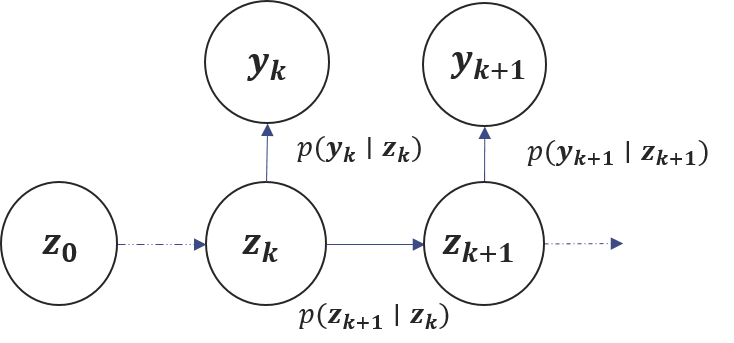
\includegraphics[width=0.5\textwidth]{hmc.png}
    \caption{Chaîne de Markov cachée}
    \label{fig:hidden_markov}
\end{figure}

On reconnait la partie inférieure du graphique présenté Figure~\ref{fig:graph_dt}.

\subsection{Estimation des paramètres du modèle par augmentation de l'état}
Nous avons supposé que le système était complètement décrit par la variable d'état $\bz$ que nous souhaitons estimé. Cependant, nous avons aussi supposé que le modèle était imparfait à cause d'erreur sur les données des paramètres de modèle. Ansi, les paramètres $\bm \theta$ ne sont pas connu avec certitude. L'estimation ou calibration de ces paramètres est possible en définissant un état augmenté $(\bz, \bm \theta)$.

Le modèle d'évolution est toutefois différent car les paramètres du modèle sont supposés constant dans le temps tel que

\begin{gather*}
    \left\{\begin{aligned}
         & \bm{z}_{k+1}      & = & \mathcal{M}(\hat{\bm{z}}_{k}) + \bm{\eta}_{k+1}    & , \\
         & \bm{y}_{k+1}      & = & \mathcal{H}(\bm{z}_{k+1}) + \bm{\varepsilon}_{k+1} & , \\
         & \bm{\theta}_{k+1} & = & \bm{\theta}_{k+1} + \bm{\xi}_{k+1}                 & .
    \end{aligned} \right.
\end{gather*}

L'ajout des paramètres dans la variable d'état a pu être utilisé pour résoudre des problème inverse sans calcul de gradient~\cite{iglesias_ensemble_2013}.

\section{Filtrage bayésien}~\label{filtrage_bayesien}

Le filtrage bayésien consiste à écrire la récurrence sur les lois de probabilité, pour estimer, en fonction des observations passées et courante $\mathcal D_k$ l'état courant $\bm z_k$ et de prédire l'état future $\bm z_{k+1}$.

Pour simplifier les notations, l'exposant $^{\mid k}$ qui conditionne la densité par les observations $\bm y_{1:N}$. La densité de l'état est initialisée par la densité a priori de l'état initial $p_{X_0}$.

Puis pour tout $k \geq 0$ les lois de probabilité sont tout d'abord propagées.

L'étape de propagation ou \textit{forecast} est obtenue grace à la loi des probabilité totales

\begin{equation*}
    p(\bm z_{k+1} \mid \mathcal D_k) = \mathbb{E}_{\bm z_k}\left[p(\bm z_{k+1} \mid  \bm z_k,\mathcal{D}_k) \mid \mathcal D_k \right] = \mathbb{E}_{\bm z_k}\left[p(\bm z_{k+1} \mid \bm z_k) \mid \mathcal D_k \right].
\end{equation*}

La loi \textit{a priori} de la $k+1$ observations peut être otenue de nouveau grace à la loi de probabilité totale

\begin{equation*}
    p(\bm y_{k+1} \mid \mathcal D_k) = \mathbb{E}_{\bm{x}_{k+1}}\left[p(\bm y_{k+1}\mid \bm x_{k+1}) \mid \mathcal D_k\right].
\end{equation*}

Après la $k+1$ observation $\bm y_{k+1}$, l'étape d'\textit{analyse}, permet grâce à la loi de Bayes de déterminer la loi \textit{a posteriori} de l'état

\begin{equation*}
    p(\bm z_{k+1} \mid \mathcal D_{k+1}) = p(\bm z_{k+1} \mid \bm y_{k+1}, \mathcal D_{k})  = \frac{p(\bm y_{k+1} \mid \bm z_{k+1} ,\mathcal D_k)  p(\bm z_{k+1}\mid \mathcal D_k)}{p(\bm y_{k+1}\mid \mathcal D_k)}.
\end{equation*}

Ainsi, les méthodes de filtrage présentent sous diverse forment ces deux étapes de propagation et de d'analyse pour mettre à jour la distribution de l'état au cours du temps et après mesure des observations.

\subsection{Propagation}
En pratique, il est difficile de réaliser la propagation de la distribution de l'état.
En effet, l'évolution du prior nécessite de propager entièrement la distribution à l'aide de l'équation de Fokker-Planck, celle-ci ne pouvant être résolue qu'en dimension faible~\cite{jazwinski_4_1970}.

Une première alternative consiste à uniquement considérer l'évolution pour les deux premiers moments. Dans ce cas, il s'agit de considérer que l'erreur de l'état $\bz_k$ suit une distribution Gaussienne $\mathcal{N} (0, \bm P_k)$. Si le modèle d'évolution $\mathcal{M} = \bM$ est linéaire, alors la matrice de covariance de l'état $\bz_{k+1}$ devient

\begin{equation*}
    \bP_{k+1} = \bM \bP_{k} \bM^T + \bm{Q_k}
\end{equation*}où $\bm Q_k$ est la matrice de covariance de l'erreur de modèle.

Cette proposition est un des éléments utilisés dans le filter de Kalman~\ref{kalman_filter}. Dans le cas où le modèle n'est pas linéaire, alors une approximation peut être obtenue par linéarisation du modèle.

Une autre possibilité consiste à utiliser un ensemble pour représenter la distribution de l'état. L'état est représenté par un ensemble d'échantillons ou particules tel que $p(\bz)  = \sum_{i=1}^{N} \omega^i \delta(\bz - \bz^i)$ est une distribution empirique de la distribution. C'est l'hypothèse qui est utilisé dans le filtre particulaire~\ref{sec:filtre_particulaire} mais également dans le filtre de Kalman d'Ensemble~\ref{sec:enkf}. Dans ce dernier cas, les membres $\bx^i$ sont supposées indépendant et identiquement distribué, ainsi les poids égaux à $1/N$.

% \subsection{Filtre particulaire}~\label{sec:filtre_particulaire}

% Le filtre particulaire est une implémentation du filtre bayésien qui approxime la PDF à l'aide d'une distribution empirique. Les transformations du filtre, \textit{forecast} et \textit{analysis} sont appliquées sur les membres de cet échantillon.
% Cette méthode converge vers la distribution exacte lorsque le nombre de particule $N \to \infty$.

% Le prior de l'état $p(\bm z)$ à l'instant $k$ est représenté par un ensemble de $N$ réalisations $\{\bm z_k^1, \bm z_k^2, \dots \bm z_k^N\}$ de tel sorte que

% \begin{equation*}
%     p_{\bm z_k}(\bm z) \simeq \sum_{i=1}^N \omega^i_k \delta(\bm x - \bm x_k^i) \quad \text{with} \sum_{i=1}^N \omega^i_k = 1, \quad \omega^i_k > 0.
% \end{equation*}

% où $\delta$ est la masse de Dirac et $\omega^i_k$ les poids associés à chaque membre. Initialement, les échantillons sont supposés tirés de manière uniforme de tel sorte que $\omega^i_k = 1/N$.

% Lors de l'étape de \textit{propagation}, les particules sont propagés par le modèle de manière déterministe.

% % Pour s'en convaincre, le loi de probabilité totale \ref{tot_rule} peut être réécrite

% % \begin{eqnarray*}
% %     p_{\bm X_{k+1}}^{\mid k}(\bm x) &=& \int p_{\bm X_{k+1}\mid \bm X_{k} = \bm x'}(\bm x) p_{\bm X_{k}}^{\mid k}(\bm x')dx' \\
% %     &\simeq& \int p_{\bm X_{k+1}\mid \bm X_{k} = \bm x'}(\bm x) \sum_{i=1}^N \omega^i_k \delta(\bm x' - \bm x_k^i) dx' \\
% %     &\simeq& \sum_{i=1}^N \omega^i_k  \int p_{\bm X_{k+1}\mid \bm X_{k} = \bm x'}(\bm x) \delta(\bm x' - \bm x_k^i) dx' \\
% %     &\simeq& \sum_{i=1}^N \omega^i_k \delta(\bm x - \mathcal M_{k,k+1}(\bm x_k^i) - \bm \eta_{k,k+1}) = \sum_{i=1}^N \omega^i_k \delta(\bm x - \bm x_{k+1}^i).
% % \end{eqnarray*}

% Quant à l'étape d'analyse, elle correspond à une mise à jour du poids de chaque membre, qui correspond à sa vraissemblance conditionnée aux données

% \begin{eqnarray*}
%     p_{\bm X_{k+1}}^{\mid k+1}(\bm x) &\propto& p_{\bm Y_{k+1} \mid \bm X_{k+1} = \bm x}^{\mid k}(\bm y)  \sum_{i=1}^N \omega^i_k \delta(\bm x - \bm x_{k+1}^i) \\
%     &\propto& \sum_{i=1}^N  \omega^i_k~p_{\bm Y_{k+1} \mid \bm X_{k+1} = \bm x_{k+1}^i}^{\mid k}(\bm y)\delta(\bm x - \bm x_{k+1}^i)
% \end{eqnarray*}

% ce qui donne

% \begin{equation*}
%     \omega^i_{k+1}  = \frac{\omega^i_k~p_{\bm Y_{k+1} \mid \bm X_{k+1} = \bm x_{k+1}^i}^{\mid k}(\bm y_{k+1}) }{\omega^j_k~\sum_j^N p_{\bm Y_{k+1} \mid \bm X_{k+1} = \bm x_{k+1}^j}^{\mid k}(\bm y_{k+1}) }
% \end{equation*}

% Où le dénominateur est simplement un terme de normalisation.

% Cependant, lorsque la dimension est grande, le nombre de poids non nulle à tendance à tendre vers 0. Pour éviter cela, des méthodes de rééchantillonnage du \textit{posterior} ont été développé. Le filtre bootstrap \cite{gordon_1993} consiste à selectionner les membres de poids les plus élevé, de les cloner de manière proportionnelle à leurs poids. Après échantillonnage, $N$ particules sont rassemblées, dont certaines sont identitiques avec des approximativement égaux.
% Un exemple d'algorithme suivant

% \begin{algorithm}
%     \caption{Implémentation du rééchantillonnage par \textit{bootstrap}.}
%     \For{membre $n$ do}{
%     Tirer $u$ dans $\mathcal{U}[0,1[$\;
%     Initialiser $j=1$\;
%     Affecter $S_w = w^1$\;
%     \While{$S_w < u$}{
%         $j = j+1$\;
%         $S_w = S_w + w(j)\;$
%     }
%     Le membre $j$  est conservé et remplace le membre $n$.
%     }
% \end{algorithm}

\subsection{Filtre de Kalman}~\label{kalman_filter}

Le filtre de Kalman introduit en 1960~\cite{kalman_new_1960} est une version du filtre Bayésien appliqué à un modèle linéaire Gaussien. Dans ces conditions, la distribution de l'état a priori de l'état et des observations sont défini par leur deux premiers moment tel que la propagation devient

\begin{eqnarray*}
    \hat{\bm{m}}_{z} &=& \bE [\bm z_{k+1} \mid \mathcal D_k] = \bm M \bm m_z,\\
    \hat{\bm  P}_{z} &=& \bV [\bm z_{k+1} \mid \mathcal D_k] = \bm M \bm m_z \bm M^T + \bm Q,
\end{eqnarray*}

et le modèle d'observation donne

\begin{eqnarray*}
    \hat{\bm{m}}_y &=& \bE [\bm y_{k+1} \mid \mathcal D_k] = \bm H \hat{\bm{m}}_{z},\\
    \bm C_{y,y}&=&\bV [\bm y_{k+1} \mid \mathcal D_k] = \bm H \hat{\bm  P}_{z} \bm H^T + \bm R, \\
    \bm C_{z,y} &=& \text{Cov}[\bm z_{k+1}, \bm y_{k+1}\mid \mathcal D_k] = \hat{\bm  P}_{z} \bm H^T,
\end{eqnarray*}

De telle sorte que la distribution \textit{a posteriori}, si cette dernière est non-dégénérée (ce qui est le cas si $\bm R$ n'est pas singulière), est défini par ses deux premiers moments qui sont

\begin{eqnarray*}
    \bm m_z &=& \bE[\bm X^{\mid k}_{k+1} \mid \bm Y_{k+1}^{\mid k}] = \hat m_X + \bm C_{X,Y} \bm C_{Y,Y}^{-1} (\bm y_{k+1} - m_Y), \\
    \bm P_{k+1} &=& \bV[\bm X^{\mid k}_{k+1} \mid \bm Y_{k+1}^{\mid k}] = \hat{\bm  P}_{k+1} - \bm C_{X,Y} \bm C_{Y,Y}^{-1} \bm C_{X,Y}^T.
\end{eqnarray*}

Ainsi la distribution a posteriori est définie comme un produit matriciel où l'estimateur a priori $\hat m_X$ et sa variance $\hat{\bm  P}_{k+1}$ sont mis à jour à partir du \textbf{gain de Kalman} $\bm K = \bm C_{X,Y} \bm C_{Y,Y}^{-1} $ et du \textbf{terme d'innovation} $(\bm y_{k+1} - m_Y)$ de telle sorte que les précédentes équations s'écrivent

\begin{eqnarray*}
    m_X &=& \hat m_X + \bm K (\bm y_{k+1} - m_Y), \\
    \bm P_{k+1} &=& (\bm I - \bm K\bm H)\hat{\bm  P}_{k+1} \\.
\end{eqnarray*}

Finalement, on peut réécrire
\begin{algorithm}
    \caption{Filtre de Kalman}
    \KwData{Initialisation de l'état $m x$ et de sa covariance $\bm P$;}
    \For{$k \geq 1$}{
        Prédiction\;
        $\hat m_x = \bm M m x $\;
        $\hat{\bm  P} = \bm M \bE [\bm X_{k+1}^{\mid k}] \bm M^T + \bm Q$\;
        Observation de $\bm Y \to \bm y$
        Analyse\;
        Calcul du gain de Kalman: $\bm K = \hat{\bm{P}}\bm H^T (\bm H \hat{\bm  P}\bm H^T + \bm R)^{-1}$ \;
        Calcul de l'analyse\;
        $m_x = \hat m_x + \bm K (\bm y - \bm H \hat m_x)$\;
        Calcul de la matrice de covariance de l'état\;
    }
\end{algorithm}

\subsection{Filtre de Kalman d'Ensemble (EnKF)}~\label{sec:enkf}

Pour surmonter les limitations du filtre de Kalman classique et du filtre particulaire, le filtre de Kalman d'ensemble (EnKF) a été développé par Evensen~\cite{evensen_sequential_1994}. L'EnKF est une méthode d'assimilation de données qui utilise un ensemble de prévisions pour estimer l'état et les incertitudes d'un système. Contrairement au filtre de Kalman classique, qui est optimal pour des systèmes linéaires et des erreurs gaussiennes, l'EnKF est plus robuste quant aux non-linéarités et aux distributions non gaussiennes.

L'EnKF fonctionne en générant un ensemble de prévisions  (ou états) $(\bx_i^f)_{i=1}^N$ à partir du modèle. Chaque membre de l'ensemble est ensuite mis à jour indépendamment en utilisant les observations disponibles. A parti de cet ensemble de représentant, supposé identiquement distribué, la matrice de covariance et la moyenne vont pouvoir être estimée.

Pour cela, nous définission la matrice d'état $\mstate_f = [\state^1, \dots, \state^N]$ et d'annomalies $\annomX_f$ dont les colonnes sont les états de chaque membre normalisé et centré ce que l'on peut écrire de la manière suivante

\begin{equation*}
    \annomX_f = \frac{1}{\sqrt{N - 1}}(\bm X_f - \overline{\state}_f \bm{1}^T),
\end{equation*}où $\bm{1} \in \mathbb{R}^N$ est un vecteur de 1.

Respectivement, la matrice d'observation et les anomalies d'observation sont $\mathcal Y_f = [\mathcal{H}(\state^1_f), \dots, \mathcal{H}(\state^N_f)]$ et $\annomY_f$, où les colonnes sont données par

\begin{equation*}
    \annomY_f = \frac{1}{\sqrt{N - 1}} \left(\mathcal Y_f - \overline{\obs}_f \bm{1}^T \right) \quad \text{avec} \quad \overline{\obs}f = \frac{1}{N} \sum{j=1}^{N} \mathcal{H}(\state^j_f).
\end{equation*}

L'ensemble définit la covariance entre les états et les observations $\Cov \bm H^T$, la covariance entre les observations $\Cov \bm H^T$, et $\tilde{\bm{K}}$

\begin{eqnarray*}
    \Cov \bm H^T &=& \frac{1}{N - 1} \sum_{i = 1}^{N} {(\state^i_f - \overline{\state}_f)}^T {\left[ \mathcal{H}_k(\state^i_f) - \overline{\bm{y}}f\right]}^T = \annomX_f \annomY_f^T, \\
    \bm H \Cov \bm H^T &=& \frac{1}{N -1} \sum{i = 1}^{N}\left[ \mathcal{H}_k(\state^i_f) - \overline{\bm{y}}_f\right] {\left[ \mathcal{H}_k(\state^i_f) - \overline{\bm{y}}_f\right]}^T = \annomY_f \annomY_f^T,\\
    \tilde{\bm{K}} &=& \Cov \bm H^T{(\bm H \Cov \bm H^T + \bm R)}^{-1} = \annomX_f \annomY_f^T {(\annomY_f \annomY_f^T + \bm R)}^{-1}.
\end{eqnarray*}

Cette implémentation sans matrice d'observation repose sur l'approximation par la méthode des sécantes $\mathcal{H}(\state^i_f - \overline{\state}_f) \approx \predi - \overline{\obs}f$.
Ensuite, la prévision est mise à jour vers un ensemble a posteriori ${[\state^i_a]}{i=1}^{N}$ tel que

\begin{equation} \label{eq:enkf_formula}
    \mstate_a = \mstate_f + \tilde{\bm{K}} ( \mdata - \mpred),
\end{equation}
où ${[\mdata]}^i = \obs + \bm{\varepsilon}^i$ est l'observation perturbée avec $\bm{\varepsilon}^i \sim \mathcal{N}(\bm{0}, \bm R) $, $\tilde{\bm{K}}$ est la matrice de gain de Kalman ensembliste et $( \mdata - \mpred)$ est le terme d'innovation.
L'étape de prévision est ensuite appliquée à l'ensemble analysé jusqu'à l'observation suivante.
Sur la base de cette formulation, nous pouvons déduire une formule de correction basée uniquement sur les prédictions des membres et les observations.

Nous pouvons réécrire la formule de mise à jour du filtre en utilisant les matrices d'anomalies précédentes.

\begin{equation*}
    \mstate_a = \mstate_f + \annomX_f \annomY_f^T {({\annomY_f \annomY_f^T + \bm R})}^{-1}(\mdata - \mpred)
\end{equation*}

Nous reformulons le terme de correction en remarquant que $ \bm{1}^T \annomY_f^T = \bm{0}$. Nous définissons $\Fcorr$, la matrice de correction qui donne la mise à jour en termes de combinaisons linéaires des états prévisionnels

\begin{equation}
    \mstate_a = \mstate_f + \mstate_f \Fcorr, \quad \Fcorr = \annomY_f^T {(\annomY_f \annomY_f^T + \bm R)}^{-1}(\mdata - \mpred).
\end{equation}

% Les équations de l'EnKF peuvent être présentées comme suit

% - **Étape de Prédiction** :
% $$x_i^f = F(x_i^a),$$
% où $x_{i}^{f}$ est la prévision du i-ème membre de l'ensemble, et $M$ est le modèle du système.

% - **Étape de Mise à Jour** :
% $$x_{i}^{a} = x_{i}^{f} + K(y_{i} - h_i^f),$$
% avec $K$ le gain de Kalman, calculé comme :
% $$K = \text{cov}(x^f, h^f)(\text{cov}(h^f, h^f) + R)^{-1}$$
% où $\text{cov}$ est l'opérateur de covariance, $(h_i^f)_{i=1}^N$ est l'ensemble d'observations prédites, et $R$ est la covariance du bruit de mesure.

Dans l'EnKF, $x_{i}^{a}$ est l'état analysé (ou mis à jour) pour le i-ème membre de l'ensemble, et $y_i$ représente les observations. Cette méthode permet de capturer la distribution de probabilité de l'état du système de manière plus efficace et avec moins de charge de calcul que le filtre particulaire, surtout dans les systèmes de grande dimension.

Cette version de l'EnKF est parfois appelé EnKF stochastique car les observations $y_i$ correspondent aux données mesurées bruitées, i.e. $y_i = y + \varepsilon_i$ où $\varepsilon_i$ correspond au bruit de mesure. Ce bruit numérique permet de supprimer un biais statistique sur l'estimation de l'état~\cite{van_leeuwen_consistent_2020}. On trouve également d'autre implémentation du filtre de Kalman d'ensemble comme le filtre EnKF déterministe comme le filtre ETKF, qui cherche une mise à jour qui permet d'obtenir une approximation de la matrice de covariance analysée du filtre de Kalman en en cherchant une racine carrée~\cite{bishop_adaptive_2001}.

\section{Méthodes variationnelles}~\label{sec:variation}
\subsection{Estimation du maximum a posteriori}

La distribution a posteriori précédemment définie permet dans un premier temps de pouvoir définir l'estimateur MAP (\textit{Maximum A Posteriori}). Il est la meilleure estimation de l'état connaissant les données mesurées. Il est défini comme

\begin{equation*}
    \bm x_{\text{MAP}} = \argmax_{\bm x} p(\bm x \mid \bm y).
\end{equation*}

Cette estimateur peut directement être déterminé directement à partir de la distribution comme avec le filtre particulaire~\ref{filtre_particulaire}.

Néanmoins, Le logarithme étant une fonction strictement croissante, la maximisation de la posterior est équivalente à minimiser $\mathcal L$. D'où la nouvelle expression de $\bm x_{\text{MAP}}$

\begin{equation*}
    \bm x_{\text{MAP}} = - \argmin_{\bm x} p(\bm x \mid \bm y).
\end{equation*}

Le MAP peut être obtenu par des méthodes d'optimisaiton numérique en fonciton de la complexité de la distribution.

Une manière de déterminer cet estimateur est d'introduire que la distribution a priori de l'état et des observations sont Gaussiennes.

Nous supposerons donc ici que les variables aléatoire introduites dans la section précédentes sont définies comme

\begin{eqnarray*}
    \bm \eta &\sim& \mathcal{N}(\bm 0, P_{k+1}), \quad p(\bm x_{k+1}) = \mathcal{N}(\bm x_{k+1}^f, P_{k+1})\\
    \bm \varepsilon & \sim & \mathcal N(\bm 0, R), \quad \quad p(\bm y_{k+1}) = \mathcal{N}(\bm g(\bm x_{k+1}^f) , R_{k+1})\\.
\end{eqnarray*}~où $\bm x_{k+1}^f = \mathcal{M}(\bx_{k})$ l'état prédit par le modèle. Nous nous interessons maintenant à l'étape de mise à jour à l'instant $k+1$, l'indice temporel sera implicite pour le reste de la section.

La distribution a posteriori peut être réécrite comme

\begin{equation*}
    p(\bm x \mid \bm y) \propto \exp\left(- \mathcal{\L}(\bm x)\right),
\end{equation*}

avec $\mathcal L(\bm x)$

\begin{equation*}
    \mathcal L(\bm x) = \frac12 \norm(\bm x - \bm x^f)_{ \bP^{-1}} + \frac12 \norm{\bm h(\bm x) - \bm d}_{\bR^{-1}}.
\end{equation*}

Le problème à minimiser devient alors

\begin{equation*}
    \bm x_{\text{MAP}} = \argmin_{\bm x} \mathcal L(\bm x).
\end{equation*}

Cette définition est à l'origine d'un ensemble de méthodes variationnelles pour l'assimilation de données dont la méthode 3DVar ou 4DVar courament utilisé en météorologie~\cite{talagrand1997assimilation}.
Le minimum de cette fonction est obtenue en annulant son gradient qui se trouve être

\begin{equation*}
    \nabla_{\bx} \mathcal L(\bx^a) = \bP^{-1} (\bx^a - \bx^f) + \nabla_{\bx^a} \bm h (\bx^a) \bR^{-1}(\bh(\bx^a) - \bm d) = \bm 0.
\end{equation*}


On peut aussi faire plusieurs remarques :

\begin{itemize}
    \item L'inverse de la dérivée seconde de la fonction coût $\mathcal L$, Hessienne, est une approximation à l'ordre 1 de la matrice de covariance a posteriori,
    \item Si l'opérateur d'observation $h$ est non linéaire alors, le problème n'est pas convexe et une méthode itérative de minimisation est souvent mis en place. Même dans le cas où $h$ est linéaire, le stockage de matrice de grande dimension peut encourager à utiliser ces méthodes itérative.
\end{itemize}

\subsection{Méthode 3DVar}~\label{subsec:3dvar}

La méthode 3DVar est un cas particulier de l'équation précédente qui permet de résoudre le problème de minimisation de la solution itérative à faible coût. Elle consiste à supposer fixe et connu les matrices de covariance $\bP$ et $\bR$. Ainsi, la matrice Hessienne $\bm B$ est donnée par $\bP$

\subsection{Equivalence avec la mise à jour de Kalman}

Elle se place dans le cas où la fonction d'observation est linéaire $\bm h(\bx) = \bH \bx$.
$$\mathcal L_{3D}(\bx) = \frac{1}{2}\norm{\bx-\bx_b}_{\bP^{-1}}^2+ \frac{1}{2}\norm{y-H(x)}^2_{R^{-1}}$$

Dans ce cas, l'annulation du gradient de la fonction coût se réduit à l'expression suivante

\begin{equation*}
    \bP^{-1} (\bx^a - \bx^f) + \bH^T \bR^{-1}(\bH \bx^a - \bm d) = \bm 0,
\end{equation*}

Ce qui nous permet d'obtenir une expression à l'estimateur MAP

\begin{equation*}
    \bx^a = \bx^f + (\bP^{-1} + \bH^T \bR^{-1} \bH)^{-1} \bH^T \bR^{-1} (\bd - \bH \bx^f),
\end{equation*}~qui est l'expression de la mise à jour dans l'espace d'état.Il peut être coûteux d'inverser la matrice $(\bP^{-1} + \bH^T \bR^{-1} \bH)^{-1}$ si l'espace d'état est de grande dimension. En appliquant deux fois la formule de Sherman-Morisson-Woodbury, si $\bP^{-1}$ et $\bR^{-1}$ sont inversibles, la mise à jour peut être réécrite dans l'espace de mesure

\begin{equation*}
    (\bP^{-1} + \bH^T \bR^{-1} \bH)^{-1} = \bP \bH^T (\bH \bP \bH^T + \bR)^{-1}
\end{equation*}

Ainsi la matrice de covariance d'état $\bP$ ne necessite pas d'être inversé. De plus on retrouve le gain de Kalman $\bK = \bP \bH^T (\bH \bP \bH^T + \bR)^{-1}$ précédemmment défini. Cette estimateur ainsi obtenu est également le BLUE (\textit{Best Linear Unbiased Estimator}). C'est en effet, l'expression est la combinaison linéaire de $\bx^f$ et $\bd$ dont l'erreur $\varepsilon^a$ est non biaisée ($\mathbb{E}[\varepsilon^a] = 0$), et dont la variance est minimale ($\Tr(\bP^a)$).

Finalement, sachant que la posterior est Gausienne, en prenant l'inverse de dérivée seconde de la fonction coût, la matrice de covariance peut être obtenue

\begin{equation*}
    (\bP^a)^{-1} = \bP^{-1} + \bH \bR^{-1} \bH^T
\end{equation*}

De nouveau avec l'identité de SMW

\begin{equation*}
    (\bm{I} - \bK \bH) \bP
\end{equation*}~qui n'est autre que la mise à jour de la covariance avec le filtre de Kalman.

\section{Méthode variationnelle d'ensemble}

\subsection{Maximum de vraissemblance échantillonné}
Les méthodes variationnelles précédemment décrite offre la possibilité de trouver le maximum d'un distribution a posteriori. Cependant, à l'aide de méthode d'ensemble, il est également possible d'estimer complètement cette distribution.

Pour cela, nous nous plaçons dans le cas d'un prior d'état Gaussien $\bm x^f$ de matrice de covariance $P^f$. On suppose $N$ échantillon i.i.d.de cette distribution $\bm x^f_i$. Après introduction de la mesure perturbée $\bm d_i = \bm d + \bm \varepsilon_i$ avec $\varepsilon_i \sim \mathcal{N}(\bm 0, \bm R)$. Alors, la distribution à posteriori peut-être échantillonnée en minimisant un ensemble de fonction coût défini pour chaque membres $i = 1, \dots, N$

\begin{equation*}
    \mathcal L_i(\bm x) = \frac12 \norm{\bm x -\bm x^f_i}^2_{\bm P^f} + \frac12 \norm{\bm h(\bm x^f_i) - \bm d_i}_{\bm R}^2,
\end{equation*}Celles-ci sont indépendantes entre chaque membre et offrent une forme similaire au MAP cette fois autour de la valeur des membres et de la mesure perturbée. Ainsi, les mêmes algorithmes de minimisation peuvent être appliqué pour résoudre ces fonctions coût.

Dans le cas linéaire et Gaussien, nous avons précedemment vu dans la Section~\ref{sec:variation} que le MAP pouvait être obtenu grâce au gain de Kalman. De même, connaissant la matrice de covariance d'état $\bm P$ et l'opérateur tangent $\bm G_i = \nabla^T_{\bx} \bm h(\bx_i)$, on obtient un ensemble de mise à jour du filtre de Kalman autour de chaque membre

\begin{equation}~\label{eq:rml-kalman}
    \bm x ^a_i = \bm x^f_i + \bm P \bm G_i^T (\bm G_i \bP \bm G_i^T + \bR)^{-1} (\bd_i - \bm h(\bx_i^f))
\end{equation}

Dans un cas non linéaire, nous pourrons traiter des cas non-linéaire pour être approchée dans un cas non Gaussien. Dans ce cas, on nous prendrons un linéarisation de la distribution a priori en estimant et ne conservant que les deux premiers moments de la distribution. C'est l'hypothèse qui est appliqué pour le filtre de Kalman d'Ensemble~\ref{sec:enkf}. De fait, cette résolution est obtenue dans un espace de représentant, offrant une optimisation dans un espace généralement de plus faible dimension.

\subsection{Méthode de rang faible}~\label{sec:faible_rang}

Nous utilisons dans cette section la même hypothèse que précédemment évoquée dans la partie sur le filtre EnKF~\ref{sec:enkf}. Il s'agit de considérer que la matrice de covariance peut etre représenté par un ensemble d'état. En fait, tout comme le filtre de Kalman et l'image du filtre 3DVar le filtre EnKF trouve une équivalence avec une approche variationnelle d'ensemble.

En utilisant les membres pour échantillonner la matrice de covariance, cela revient à chercher la solution dans l'espace vectoriel engendré par les membres.

En reprenant la formule~\ref{eq:rml-kalman}, et en remplaçant $\bm P \approx \annomX_f \annomX_f^T$, on obtient d'une part la mise à jour du filtre EnKF~\ref{enkf_formula}, d'autre part que l'on puis reformuler le terme de correction the correction term en définissant $\Fcorr$,

\begin{equation}
    \mstate_a = \mstate_f + \mstate_f \Fcorr, \quad \Fcorr = \frac{1}{\sqrt{N-1}} \annomY_f^T {(\annomY_f \annomY_f^T + \bm R)}^{-1}(\mdata - \mpred).
\end{equation}.

Ceci nous renseigne sur plusieurs choses:
\begin{itemize}
    \item La mise à jour du filtre EnKF est une combinaison linéaire des membres ;
    \item Il suffit de déterminer $N \times N$ pour résoudre le problème de mise à jour ;
    \item La mise à jour est indépendante pour les $N$ fonctions à minimiser ce qui permet de grandement paralléliser les problèmes d'optimisation.
\end{itemize}

Les $N$ problème de minimisation peuvent être reformulés à l'aide des termes de cette matrice $F$

\begin{equation*}
    \bm f_i = \argmin_{f \in } \frac12 \norm{\bm d - \bm h(\mstate_f + \mstate_f \Fcorr)}^2_{\bm R^{-1}} + \frac12 \norm{\bm f}_2^2
\end{equation*}

En effet \mycolor{mettre la formule ici}.

\section{Bilan du chapitre}
%classification des filtres

Celles-ci diffèrent par un certains nombres d'hypothèses que nous avons regroupé dans la Table et représenté sur la Figure
\mycolor{Faire un schéma des différentes méthodes de filtrage avec les hypothèses associées.}

Nous avons proposer différentes formulation du problème de filtrage. Après un rappel de la formulation bayésienne du problème, nous avons montrer que des formulations séquentielles

Dans les parties suivantes, nous présenterons quatres familles de méthode de filtrage.

\mycolor{présenter les différentes méthodes}
\begin{itemize}
    \item le filtre particulaire - filtre bayésien non linéaire sur distributions empirique
    \item filtre de Kalman - filtre bayésien modèle linéaire, distributions gaussienne
    \item Méthode Variationnelle d'ensemble - filtre non linéaire, distribution gaussienne
    \item filtre de Kaman d'Ensemble - filtre non linéaire, distribution gaussienne

\end{itemize}

